\documentclass{article}
\newcommand{\ii}{{\bf i}}
\newcommand{\jj}{{\bf j}}
\newcommand{\kk}{{\bf k}}
\newcommand{\id}{{\bf 1}}
\newcommand{\hur}{\frac{\id+\ii+\jj+\kk}{2}}%The "Hurwitz point"
\newcommand{\hurwitz}{\Z\left[\hur,\ii,\jj,\kk\right]}%The set of Hurwitz integers
\usepackage[utf8]{inputenc}
\usepackage[dvips]{graphicx}
\usepackage{a4wide}
\usepackage{amsmath}
\usepackage{euscript}
\usepackage{amssymb}
\usepackage{amsthm}
\usepackage{amsopn}
\usepackage[colorinlistoftodos]{todonotes}
\usepackage{graphicx}

\usepackage{ulem}
\usepackage{xcolor}
\newcommand{\cs}[1]{\color{blue}{#1}\normalcolor}

%Matrix commands
\newcommand{\ba}{\begin{array}}
\newcommand{\ea}{\end{array}}
\newcommand{\bmat}{\left[\begin{array}}
\newcommand{\emat}{\end{array}\right]}
\newcommand{\bdet}{\left|\begin{array}}
\newcommand{\edet}{\end{array}\right|}

%Environment commands
\newcommand{\be}{\begin{enumerate}}
\newcommand{\ee}{\end{enumerate}}
\newcommand{\bi}{\begin{itemize}}
\newcommand{\ei}{\end{itemize}}
\newcommand{\bt}{\begin{thm}}
\newcommand{\et}{\end{thm}}
\newcommand{\bp}{\begin{proof}}
\newcommand{\ep}{\end{proof}}
\newcommand{\bprop}{\begin{prop}}
\newcommand{\eprop}{\end{prop}}
\newcommand{\bl}{\begin{lemma}}
\newcommand{\el}{\end{lemma}}
\newcommand{\bc}{\begin{cor}}
\newcommand{\ec}{\end{cor}}

%sets of numbers
\newcommand{\N}{\mathbb{N}}
\newcommand{\Z}{\mathbb{Z}}
\newcommand{\Q}{\mathbb{Q}}
\title{Abstract Algebra}
\author{August, Evelyn}
\date{5/9/2021}
\maketitle
\begin{document}
\fbox{Ch0, #12} Show that 5n+3 and 7n+4 are relatively prime for all n.\\

\fbox{proof}
We know that, if a and b are relatively prime, the greatest common divisor of a and b, gcd(a,b), is 1. By applying the Euclidean Algorithm we get: 
$$\gcd(5n+3, 7n+4)=\gcd(2n+1, 5n+3)=\gcd(3n+2, 2n+1)=\gcd(n+1, 2n+1)=\gcd(n, n+1)=\gcd(1, n)=1 $$
Hence, 5n+3 and 7n+4 are relatively prime for all n. Q.E.D.
\\

\\

\fbox{Ch1, #24}
For each design below, determine the symmetry group (ignore imperfections). 
\begin{figure}[htbp]
\centerline{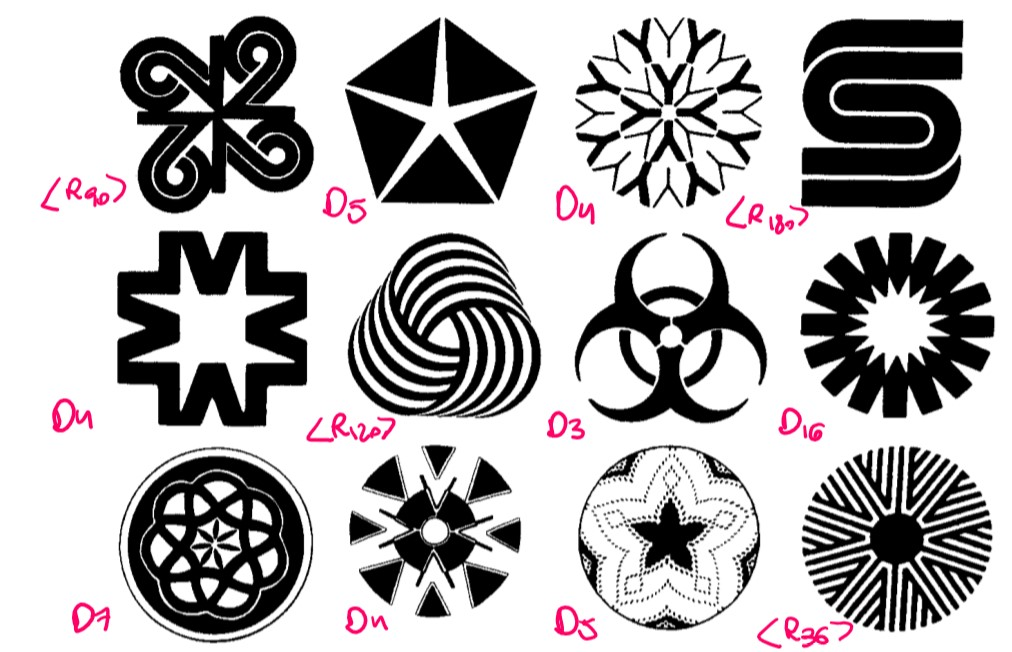
\includegraphics[scale=0.5]{symmetry_groups.jpg}}
\caption{}
\label{fig}
\end{figure}\\



\\
\\
\fbox{Ch2, #19} Prove that the set of all 2x2 matrices with entries from R and determinant +1 is a group under matrix multiplication.\\

\fbox{proof}\\
1) The set is non-empty, since, for example, the identity matrix is one element of the set. \\
2) The matrix multiplication is a closed, binary operation on this set, since the product again is a 2x2 matrix with real entries. Also, if A and B are elements of the set, then $\det(A)=\det(B)=+1$. Furthermore, $\det(AB)=\det(A)\cdot\det(B)=+1$\\
3) The identity element e is the identity matrix $I= \begin{pmatrix}
1&0\\
0&1
\end{pmatrix}$, since $A\cdot I = I\cdot A=A$ for all matrices A in the set.\\
4) Every element A of the set has an inverse $A^{-1}$, since every square matrix with determinant +1 is invertible. \\
5) Matrix multiplication is associative. \\

Hence, the set of all 2x2 matrices with real entries and determinant +1 is a group under matrix multiplication. \\

\\
\fbox{Ch2, #47} Show that if in a group there is a rule that any square of an element is the identity, then it follows that that group is Abelian.\\

\fbox{proof}
Let $G$ be a group, and let $a$ and $b$ be elements of that group. Suppose that the square of any element in $G$ is the identiy, $e$. Then by closure and the definition of $G$, behold, we have
$$(a*b)^2 = e.$$
Furthermore, $a*(a*b)^2 = a*e = a.$ As groups are associative, we have $$a*a*b*a*b = a = (a*a)*b*a*b = b*a*b.$$ Multiplying $b$ on the right, we have 
$$b*a*b*b = a*b = b*a*(b*b) = b*a*e = b*a.$$ Hence we have $b*a = a*b.$ Q.E.D.\\
\newpage
\fbox{Ch2, #37} Let $G$ be a finite group. Then the number of elements $x$ such that $x^3 = e$ is odd, and the number of elements $y$ such that $y^2 \ne e$ is even.\\

\fbox{proof} Let $|G|$ be the order of $G$. \\
\begin{itemize}
    \item Suppose that there is a subset of $G$, $S$, such that each element $x\in S$ has the property that $x^3 = e$. Clearly $e$ is a member of this group, as $e$ raised to any power must be $e$. Let $x$ be an arbitrary element of $S$ not equal to $e$. Since $x^3 = e$, by the associative law of groups, $x(x^2) = e$, hence $x^{-1} = x^2$. Furthermore, by the uniqueness property of the inverse in groups, $x^2 \ne x$. Furthermore, $(x^2)^3 = x^6 = x^3x^3 = 1$, hence $x^2$ is another element of $S$. Since for each element of $S$ not $e$, there is a pair element of $S$ corresponding to it, the order of $S$ must be $2n + 1$, so the number of elements in a finite group $x$ such that $x^3 = e$ is odd.
    \item Let $S$ be a subset of $G$ such that each element $x\in S$ has the property that $x^2 \ne e$. Note that $S$ could be empty, in which case the proposition holds. Suppose then that $S$ is not empty. Let $x$ be an arbitrary element of $S$. By the associative, it is clear that $(x^{-1})^2x^2 = x^{-1}x^{-1}xx = x^{-1}(x^{-1}x = e)x = e$, hence $(x^{-1})^2 = (x^2)^-1$. Furthermore, since $x^2 \ne e$, it follows that $(x^{-1})^2x^2 \ne (x^{-1})^2 e$, hence $e\ne (x^{-1}^2)$. Furthermore, $x^{-1}$ is distinct from $x$, as $x^2 \ne e$. Hence it follows that for each element $S$, there is exactly one more element in $S$. In other words, $|S|$ has cardinality $2n$, so there are an even number of elements $x$ in $G$ such that $x^2 \ne e$
\end{itemize}
\end{document}